\documentclass[10pt,sigconf,letterpaper,anonymous,nonacm]{acmart}

\usepackage{booktabs}
\usepackage{graphicx}
\usepackage{xspace}
\usepackage{balance}
\usepackage[htt]{hyphenat} % allow hyphenation in \texttt
\usepackage{adjustbox}

\emergencystretch=1em  % allow slightly looser spacing to avoid overfull hboxes

\newcommand{\sysname}{Browse\-Trace\xspace}
\newcommand{\release}{\texttt{release-v3}\xspace}
\newcommand{\submissioninfo}{Paper \#85, 13 pages body, 16 pages total}

\hyphenation{Browser-Use load-bal-anc-ing}

%% Rights and DOI metadata (required by acmart; left blank for submission)
\setcopyright{none}
\settopmatter{printacmref=false,printfolios=true}
\renewcommand\footnotetextcopyrightpermission[1]{}
\acmConference[IMC '26]{ACM Internet Measurement Conference}{October 2026}{Karlsruhe, Germany}
\acmYear{2026}
\acmDOI{}
\acmISBN{}
\acmPrice{}

\begin{document}
\pagestyle{plain}  % IMC requires page numbers on review submissions

\title{BrowseTrace: Request-Level Traffic Characterization of Browser-Mediated AI Agents}
\author{Anonymous Author(s)}
\affiliation{\institution{Anonymous Institution}}
\makeatletter
\gdef\addresses{\@author{\submissioninfo}}
\gdef\authors{Anonymous Author(s)}
\makeatother

%% CCS concepts (required by acmart)
\begin{CCSXML}
<ccs2012>
<concept>
<concept_id>10003033.10003083</concept_id>
<concept_desc>Networks~Network measurement</concept_desc>
<concept_significance>500</concept_significance>
</concept>
<concept>
<concept_id>10002951.10003260.10003282</concept_id>
<concept_desc>Information systems~Web applications</concept_desc>
<concept_significance>300</concept_significance>
</concept>
<concept>
<concept_id>10010520.10010575.10010755</concept_id>
<concept_desc>Computer systems organization~Cloud computing</concept_desc>
<concept_significance>300</concept_significance>
</concept>
</ccs2012>
\end{CCSXML}

\ccsdesc[500]{Networks~Network measurement}
\ccsdesc[300]{Information systems~Web applications}
\ccsdesc[300]{Computer systems organization~Cloud computing}

\keywords{web measurement, browser automation, AI agents, caching, benchmark, reproducibility}

\begin{abstract}
AI agents that browse the real web are a new user class, yet no
public dataset captures their HTTP traffic.  We present \sysname, a
reproducible HTTP-level benchmark of AI-agent browser behavior.
Using Chrome DevTools Protocol instrumentation, we collect
1{,}301~sessions: 901~agent-driven runs spanning six LLMs from five
providers (GPT-4.1-mini, Gemini~2.5 Flash and Pro, Claude~Haiku~4.5,
DeepSeek-V3.2, and Alibaba's Qwen~2.5-Coder~7B), paired with a
400-session scripted baseline across four regions.  On identical
tasks, LLM agents issue 2--5$\times$ more HTTP requests than the
scripted baseline, with per-task amplification reaching 26$\times$
for open-ended prompts.  Rendering dominates payloads: scripts and
stylesheets jointly carry 69\% of transferred bytes versus 2.9\% for HTML.
Replaying 82{,}455~scripted requests and 357{,}782~LLM-driven
requests under \texttt{libCacheSim} through six cache policies,
size-aware eviction (GDSF) outperforms LRU at edge-cache sizes: at
5\,MiB, GDSF reaches 59.5\% hit rate vs.\ 37.4\% on scripted traffic
and 76.2\% vs.\ 43.5\% on LLM-driven traffic.  Policy rankings diverge from
those reported for production human-browsing traces.  We release
traces, a cache-simulator schema, and replay tooling for measurement
and CDN research.
\end{abstract}

\maketitle

%% ====================================================================
\section{Introduction}
\label{sec:intro}

A new class of web workloads is emerging.  Browser-mediated AI
systems (ranging from deterministic scripted drivers to LLM-steered
autonomous agents) navigate, extract, compare, and verify information
across multiple websites within bounded sessions.  Unlike classical
crawlers that fetch individual URLs, these systems exercise the full
browser stack: they trigger JavaScript execution, load stylesheets and
fonts, follow redirects, and issue sequences of dependent fetches that
resemble human browsing sessions more than traditional bot
traffic~\cite{zhang2025}.

Concrete deployed systems in this class include OpenAI's Operator and
ChatGPT Agent~\cite{openai2025operator,openai2025chatgptagent},
Anthropic's Claude Computer Use~\cite{anthropic2024computeruse}, and
Google DeepMind's Project Mariner~\cite{google2024mariner}; \sysname
targets the HTTP footprint this class generates.
These workloads have operational significance.  Production CDN
operators report that automated traffic now constitutes a substantial
fraction of total requests~\cite{cloudflare2024bots}, and recent work
demonstrates that even simplified AI traffic models can sharply degrade
cache effectiveness~\cite{zhang2025}.
Operators report concrete impact: Wikimedia~\cite{wikimedia2025crawlers} saw a 50\% rise in backend bandwidth from AI scrapers, Read the Docs~\cite{readthedocs2024} logged a single crawler downloading 73\,TB of HTML in one month, and Cloudflare~\cite{cloudflare2025radar} attributes 4.2\% of HTML-request traffic to non-Google AI crawlers. Automated bot traffic accounts for roughly one third of web requests overall~\cite{imperva2024}.
Yet the research community lacks
the most basic prerequisite for rigorous study: a public, reproducible
benchmark that captures browser-mediated agent behavior at the HTTP
request level.

This gap blocks three lines of work: measurement researchers need
shared trace artifacts, systems researchers need replayable request
streams for caching and load-balancing evaluation, and
agent-benchmarking researchers need a common infrastructure-level
substrate to relate task-completion improvements to network cost.
Currently, all three rely on private traces, synthetic models, or
task-level metrics that omit request-level details.

This paper addresses the gap with \sysname, a benchmark framework
designed around real browser execution, a common trace schema, and
replay-ready exports.  The contribution is not a new task-success
leaderboard or a new cache algorithm; it is a public, request-level,
replay-ready corpus of real browser-mediated agent traffic.  We make
four contributions:

\begin{enumerate}
\item A \textbf{benchmark design} that couples
  Browser\-Use-backed browser execution with a shared
  request-level trace schema and synchronized output artifacts
  (Section~\ref{sec:design}).

\item A \textbf{public release} \release, a named manifest aggregating
  1{,}301~sessions (400~scripted-random across 4~regions; 901~LLM-driven
  across six models from five providers) plus the stitched cache-replay
  CSVs used for all quantitative claims (Section~\ref{sec:methodology}).

\item \textbf{Cross-cutting observations} on workload heterogeneity,
  geographic variation, payload composition, request timing, and
  a scripted-vs-LLM comparison showing 2--5$\times$ request
  amplification across six models
  (Section~\ref{sec:observations}).

\item A \textbf{cache replay study} on the full 82{,}455-request
  geo-distributed trace: GDSF outperforms recency-based policies on
  mixed multi-tenant traffic at per-shard/microcache sizes
  (1--50\,MiB), with a 3$\times$ object-hit-rate advantage at 1\,MiB
  narrowing at larger sizes (per-task single-tenant gap is 7.3\,pp at
  10\,MiB), showing that agentic workloads produce different cache
  policy rankings than human web traffic at this scope (Section~\ref{sec:replay}).
\end{enumerate}

\sysname unifies two execution modes under one measurement framework.
The scripted-random component is a \emph{deterministic stress-test
driver}, not a proxy for human or agent behavior, but a reproducible,
credential-free load pattern against which LLM-driven agent traffic
can be contrasted; the 2--5$\times$ amplification ratio we report is
thus relative to this synthetic floor, not to measured human browsing.  The LLM-driven component spans frontier
closed-source, agent-trained, and open-weight tiers (six models, five
providers).  This is a measurement benchmark over the agent-traffic
workload class, not a task-completion leaderboard in the sense of
WebArena or AgentBench~\cite{webarena,agentbench}; we use
\emph{browser-mediated AI agent} throughout to denote any system that
controls a real browser to complete web tasks.  The 1{,}301-session
corpus is sized for initial workload characterization and cache-policy
ranking, not production capacity extrapolation; the release protocol
supports adding sessions without invalidating prior artifacts.

The paper is organized as follows.
Section~\ref{sec:related} surveys related work across agent benchmarking,
web measurement, and cache research.
Section~\ref{sec:design} describes the benchmark design.
Section~\ref{sec:methodology} details the collection methodology and
first release.
Sections~\ref{sec:observations} and~\ref{sec:replay} present
release-level observations and a cache replay demonstration.
Section~\ref{sec:artifact} discusses artifact design.
Section~\ref{sec:discussion} draws implications for operators and
researchers, and Section~\ref{sec:limitations} addresses limitations
and planned extensions.

%% ====================================================================
\section{Background and Related Work}
\label{sec:related}

\paragraph{AI-era web traffic.}
Zhang et al.~(SoCC 2025)~\cite{zhang2025} use synthetic AI-traffic
overlays on production CDN traces to show that AI-originated request
patterns reduce cache hit rates under mixed workloads, motivating
workload-aware cache designs.
Cloudflare's 2024 bot report~\cite{cloudflare2024bots} confirms that
automated requests now constitute a large and growing share of global
web traffic.  These studies establish that agentic
traffic matters operationally, but none provides a public,
task-structured, replay-ready benchmark.

\paragraph{Browser bot detection.}
Iliou et al.~\cite{iliou2019advanced} study the boundary between human
and automated browser traffic from a detection perspective.
Industry reports~\cite{imperva2024} estimate that automated bot traffic
now exceeds 30\% of all web requests, with ``advanced bots'' that
mimic human behavior comprising a growing fraction.
Classical crawler workload characterization~\cite{arlitt2000} establishes
that traditional bots exhibit breadth-first URL-frontier access patterns
with high temporal locality.  Recent work deploys coarse-grained browser fingerprints at scale~\cite{kalantari2024browserpolygraph} and shows that evasive bots alter fingerprint attributes to escape commercial defenses~\cite{venugopalan2025fpinconsistent}.  Browser-mediated agents differ: they
produce traffic structurally similar to human sessions, making
request-level characterization essential.

\paragraph{Agent benchmarks.}
The agent-evaluation community has produced numerous benchmarks for
task-completion capabilities (Mind2Web~\cite{mind2web},
WebArena~\cite{webarena}, WebVoyager~\cite{webvoyager},
VisualWebArena~\cite{visualwebarena}, OSWorld~\cite{osworld},
AgentBench~\cite{agentbench}).  Early LLM web interaction work such as WebGPT~\cite{nakano2021webgpt} focused on question-answering quality rather than network-level characterization.
These benchmarks focus on \emph{what} agents
accomplish, not \emph{how} their behavior manifests at the network
level.  None publishes request-level HTTP traces suitable for systems
research.

\paragraph{Web measurement.}
Butkiewicz et al.~\cite{butkiewicz2011} measure website complexity,
Ihm and Pai~\cite{ihm2011} characterize web traffic composition
evolution, and Gill et al.~\cite{gill2007} characterize YouTube
traffic.  The HTTP Archive~\cite{httparchive} provides longitudinal
web page composition data, but HTTP Archive captures
isolated single-page loads from a stateless crawler.  In contrast,
\sysname captures multi-page, task-driven sessions where the agent
navigates across pages, producing temporal reuse patterns
(backtracking, revisits, shared sub-resources across navigation steps)
that single-page crawls cannot exhibit.  Ruth et al.~\cite{ruth2022toppling} examine the representativeness
of top-list-driven web measurement.  Annamalai et al.~\cite{annamalai2025beyondcrawl} show that automated crawls miss browser behaviors triggered only under realistic user interactions.
This body of work provides the methodological template for web
measurement but does not address browser-mediated agentic workloads.

Concurrent work addresses adjacent questions. Sayyid-Ali et al.~\cite{sayyidali2026sustainable} measure real-time fetching by ChatGPT and Claude over 1{,}000 queries but study answer-engine pipelines, not browser-agent sessions. Borysenko~\cite{borysenko2026devexp} identifies HTTP behavioral signatures of coding agents on documentation portals but does not collect full session traces or evaluate cache behavior. At IMC~2025, Kim et al.~\cite{kim2025robots} and Liu et al.~\cite{liu2025somesite} study AI crawler robots.txt compliance and site-operator responses, establishing the governance backdrop for agentic traffic measurement. \sysname differs from all of these: it captures real browser-agent HTTP traces at request granularity, preserves full request waterfalls and sub-resource fetches, and releases synchronized replay artifacts rather than only overlays, coarse logs, or task-level outcomes. More broadly, no public dataset provides human browsing traces at HTTP request granularity; existing releases are either automated crawls, URL-visit aggregates, or unreleased private collections (Appendix~\ref{sec:appendix-human}).

\paragraph{Cache replacement policies.}
Megiddo and Modha~\cite{megiddo2003} introduce ARC, a self-tuning
policy that balances recency and frequency.
Einziger et al.~\cite{einziger2017} propose TinyLFU, a lightweight
frequency-based admission filter.
Yang et al.~\cite{yang2023s3fifo} show that a carefully structured FIFO
queue (S3-FIFO) can outperform LRU with lower overhead;
SIEVE~\cite{yang2023sieve} further simplifies lazy-promotion eviction.
Beckmann et al.~\cite{lhd2018} propose LHD, which estimates per-object
hit density to guide eviction.
Berger et al.~\cite{berger2017} present AdaptSize, which optimizes
object admission in CDN caches.
Yang et al.~\cite{yang2023glcache} introduce GL-Cache, a
group-level learned cache replacement policy.
Waldspurger et al.~\cite{waldspurger2017} demonstrate that miniature
simulations can efficiently predict cache behavior.
These results motivate workload-specific evaluation: policy rankings
depend on request-stream characteristics, and agentic workloads may
exhibit different reuse patterns than human browsing.

\paragraph{Browser automation.}
\sysname uses BrowserUse~\cite{browseruse} (built on
Playwright~\cite{playwright}, or equivalently Puppeteer, for browser automation) as the execution substrate, chosen for
its native support of both scripted and LLM-driven modes.

\paragraph{Traffic characterization methodology.}
Like Butkiewicz et al.~\cite{butkiewicz2011}, we instrument the
browser to capture the full request waterfall.  Like Ihm and
Pai~\cite{ihm2011}, we design for repeated releases.  The key
difference is the workload source: we instrument browser-mediated AI
automation rather than human browsing or crawler traffic.

\paragraph{Agent-publisher interaction.}
The emerging ecosystem for structured agent-publisher interaction
includes TollBit~\cite{tollbit2024} for content monetization,
x402~\cite{x402} for HTTP-level payments, the robots exclusion
protocol (RFC 9309~\cite{robotstxt}) as the legacy coordination
mechanism, and the 2025 Web Bot Auth
effort~\cite{cloudflare2025signedagents,ietf2025webbotauth}, which
pushes toward cryptographic agent identity via signed HTTP requests.
None of these provides a public trace corpus for systems research.  The WebLINX dataset~\cite{weblinx} captures human
demonstrations of web tasks with full observation data, but focuses
on task structure rather than HTTP-level traffic.  SWE-bench~\cite{swebench}
evaluates agents on code repositories, not web interactions.
\sysname fills the gap between agent benchmarks (task-level) and
web measurement (request-level) by providing public traces of
browser-mediated agent HTTP traffic.

\paragraph{Positioning.}
Table~\ref{tab:positioning} summarizes the gap that \sysname addresses.
Existing agent benchmarks measure task success, not network behavior.
Web measurement work characterizes human and crawler traffic, not
agentic sessions.  Cache research evaluates algorithms on legacy
workloads (CDN production traces, storage block traces) that predate
the browser-mediated agent workload class.  \sysname sits at the
intersection: it produces request-level traces from real
browser-mediated agent sessions that are directly replayable into
systems experiments.

\begin{table}[t]
\centering
\footnotesize
\caption{Positioning of \sysname relative to existing work.
  ``Agent HTTP traces'' means request-level HTTP captures from
  browser-mediated agent sessions specifically; industry AI-bot
  reports and \cite{zhang2025} provide only aggregate or synthetic-overlay
  coverage.  $\checkmark$ = addressed, $\circ$ = partial, -- = not addressed.}
\label{tab:positioning}
\begin{tabular}{@{}lcccc@{}}
\toprule
& \textbf{Task} & \textbf{Agent HTTP} & \textbf{Multi-} & \textbf{Replay} \\
& \textbf{eval} & \textbf{traces}     & \textbf{LLM}    & \\
\midrule
Agent benchmarks               & $\checkmark$ & --               & $\circ$ & --           \\
Web measurement                & --           & --               & --      & $\circ$      \\
Cache policy work              & --           & --               & --      & $\checkmark$ \\
Industry AI-bot reports        & --           & $\circ$ (aggr.)  & --      & --           \\
Prod.-AI traffic~\cite{zhang2025} & --        & $\circ$ (synth.) & --      & --           \\
\textbf{\sysname}              & --           & $\checkmark$     & $\checkmark$ & $\checkmark$ \\
\bottomrule
\end{tabular}
\end{table}

%% ====================================================================
\section{Benchmark Design}
\label{sec:design}

\sysname is designed around four goals: real execution, common
representation, reproducibility, and systems utility.

\subsection{Real Execution}

All traces are collected from a real browser session rather than
synthesized from a model or inferred from server logs.  BrowserUse
provides the browser automation substrate, and instrumentation is
attached at the CDP layer to capture the full browser fetch pattern,
including JavaScript-triggered sub-resource loads, stylesheet fetches,
font downloads, and redirect chains.  This ensures that traces reflect
the actual request sequences that web infrastructure must handle, not an
idealized subset.

\subsection{Common Representation}

A single request-level trace schema spans collection, analysis, and
replay.  Each request record contains 32 fields organized into four
groups: (1)~\emph{request context}: timestamp, URL, HTTP method,
initiator type, resource type, redirect count, session and task
identifiers, access mode; (2)~\emph{response metadata}: status code,
content type, encoded body size, remote IP, protocol (h1.1/h2/h3),
connection reuse flag; (3)~\emph{HTTP headers}: \texttt{Cache-Control},
\texttt{ETag}, \texttt{Age}, CDN cache-status
(\texttt{X-Cache}/\texttt{CF-Cache-Status}), plus the full verbatim
response header map; and (4)~\emph{timing}: DNS, TLS, TCP, TTFB, and
transfer latency, each in milliseconds.  A replay-oriented cache key
and object size field support direct input to cache simulators.  Agent
metadata (framework version, driver type) is included at the session
level.

\subsection{Collection Modes}

The benchmark design supports two collection modes:
\begin{itemize}
\item \textbf{Controlled surface:} a local test publisher for
  head-to-head comparison between browser scraping and structured
  agent-specific access modes.
\item \textbf{Live surface:} real BrowserUse sessions against public
  websites, producing traces under production web conditions.
\end{itemize}
This paper focuses exclusively on the live collection mode.  The controlled
mode is relevant for follow-on systems work comparing access modes
but is outside the scope of the current measurement release.

\subsection{Benchmark Dimensions}

The full benchmark is designed to vary along five axes:
\begin{enumerate}
\item \textbf{Execution mode:} scripted baselines and LLM-driven agent
  runs, enabling comparison of deterministic and stochastic navigation.
\item \textbf{Task family:} aggregation, comparison, verification,
  lookup, and multi-step retrieval tasks that exercise different
  navigation patterns.
\item \textbf{Publisher mix:} news, documentation, API, regulatory, and
  reference sites with different content structures and caching
  behaviors.
\item \textbf{Geography:} repeated collection from multiple regions to
  capture CDN and localization effects.
\item \textbf{Artifact surface:} synchronized outputs feeding
  measurement, replay, and dashboard analysis from a single collection
  pass.
\end{enumerate}

The current release covers all five axes: scripted-random and
LLM-driven execution across 10~task families targeting diverse
publishers, collected from 4~geographic regions with synchronized
output artifacts.

\subsection{Output Artifacts}

Each task directory in a release contains four synchronized outputs
derived from the same collection pass:
\begin{itemize}
\item \texttt{traces.json}: full-fidelity request/response records
  for detailed analysis, including per-request timing, response
  headers, and session context.
\item \texttt{cache\_trace.csv}: a cache-simulator-ready extract
  with timestamp, cache key, and object size, following the format
  conventions used by standard cache simulation frameworks.
\item \texttt{access\_log.jsonl}: a log-format export for dashboard
  ingestion and streaming analysis, compatible with common log
  aggregation tools.
\item \texttt{summary.json}: per-task release metadata including
  aggregate statistics, collection parameters, and provenance
  information.
\end{itemize}

All four outputs are derived from the same collection pass, ensuring
consistency.  The \texttt{summary.json} manifest records exact counts
and checksums as an integrity anchor.

%% ====================================================================
\section{Methodology and Release}
\label{sec:methodology}

\subsection{Release Scope}

The release manifest \release enumerates the scripted subtree under
\texttt{releases/}, the per-model LLM session bundles in
\texttt{round9/} and \texttt{round10-*/}, and the two stitched
cache-replay CSVs (scripted and LLM).  All paths are pinned in
\texttt{artifact\_snapshot.json}.  The named release directory
contains the scripted Zurich release subset;
the full 1{,}301-session paper corpus is defined by the manifest via
the per-model bundles and the stitched canonical CSVs.

\paragraph{Task families.}
\begin{itemize}
\item \textbf{News aggregation:} breadth-first navigation across
  technology news sites (TechCrunch, The Verge, Ars Technica).
\item \textbf{API comparison:} multi-site comparison of weather API
  providers (OpenWeatherMap, WeatherAPI, Open-Meteo).
\item \textbf{Fact checking:} multi-source verification against EU
  regulatory sources (EUR-Lex, EC Digital Strategy).
\item \textbf{Regulatory lookup:} depth-first single-site navigation
  within GDPR reference material.
\item \textbf{Product comparison:} depth-first multi-site comparison
  of cloud GPU providers (AWS, GCP, Azure).
\item \textbf{Literature review:} sequential multi-page navigation
  on arXiv and Google Scholar.
\item \textbf{Travel planning:} parallel multi-page browsing across
  flights, hotels, and tourism sites.
\item \textbf{Job market:} breadth-first exploration of job listing
  platforms (Indeed, Jobs.ch, Glassdoor).
\item \textbf{Real estate:} depth-first multi-page navigation
  across apartment listing sites (Homegate, ImmoScout24).
\item \textbf{Doc.\ lookup:} depth-first navigation within
  technical documentation (Python docs, MDN).
\end{itemize}

\paragraph{Execution mode.}
The canonical corpus includes two execution modes.  The \emph{scripted-random}
driver navigates target sites with randomized link selection, producing
a reproducible, credential-free baseline (400~sessions across
4~regions).  The \emph{LLM-driven} mode covers all 10~task families
using six models from five providers (901~sessions, 357{,}782~requests
in total); the per-model scope, per-capability-tier breakdown, and
cross-model comparison appear in Section~\ref{sec:obs-llm}.

\paragraph{Geographic distribution.}
Sessions are collected from 4~vantage points: a local workstation
in Zurich (Switzerland) and Google Cloud VMs in US~Central
(Iowa, \texttt{us-central1}), Europe~West (Belgium,
\texttt{europe-west1}), and Asia~Southeast (Singapore,
\texttt{asia-southeast1}).  Each region runs the same 10~task
families with 10~scripted-random repeats, capturing CDN edge
behavior, latency variation, and region-specific content
differences.

\paragraph{Scale.}
The scripted-random component contains 400~sessions (10~task families,
10~repeats, 4~regions), producing 168{,}067~requests and 2.1\,GiB.
The initial LLM-driven component adds 300~Zurich sessions across three
models, producing 158{,}231~requests; cross-model and multi-region
extensions (Section~\ref{sec:obs-llm}) add 601~further LLM sessions,
bringing the canonical corpus to 1{,}301~sessions and approximately 526K
requests.  The Zurich sessions include enriched per-request metadata
(timing breakdown, response headers, connection details); the cloud
sessions provide the geographic dimension.

\subsection{Summary Statistics}

Table~\ref{tab:release} summarizes the release.  Confidence intervals
are computed from per-task repeats using the $t$-distribution at the
95\% level.

\begin{table}[t]
\centering
\footnotesize
\caption{Per-task summary for the Zurich scripted subset within
  \release (10~repeats each).  Mean values with 95\% CIs
  (Student's $t$-distribution, $\mathrm{df}=9$); the aggregate row
  reports the full 400-session scripted corpus.}
\label{tab:release}
\begin{tabular}{@{}lrrl@{}}
\toprule
\textbf{Task family} & \textbf{Req/run} & \textbf{MiB/run} & \textbf{Uniq.} \\
\midrule
News aggregation      & $366.9 \pm ~8.4$ & $9.64 \pm 0.16$ & $0.925$ \\
Product comparison    & $251.4 \pm ~3.0$ & $7.86 \pm 0.03$ & $0.895$ \\
Travel planning       & $254.0 \pm 29.9$ & $6.71 \pm 0.41$ & $0.859$ \\
Job market            & $206.6 \pm 30.4$ & $3.69 \pm 0.47$ & $0.905$ \\
Documentation lookup  & $124.4 \pm ~1.5$ & $0.81 \pm 0.05$ & $0.992$ \\
API comparison        & $114.2 \pm ~6.7$ & $1.72 \pm 0.23$ & $0.980$ \\
Fact checking         & $~86.8 \pm ~0.9$ & $2.92 \pm 0.01$ & $0.899$ \\
Regulatory lookup     & $~39.0 \pm <0.1$ & $1.05 \pm 0.00$ & $1.000$ \\
Literature review     & $~24.0 \pm ~0.7$ & $0.34 \pm 0.02$ & $1.000$ \\
Real estate           & $~16.0 \pm <0.1$ & $0.08 \pm 0.00$ & $0.875$ \\
\midrule
\textbf{Aggregate}    & \multicolumn{3}{l}{400 sess.\ (4 reg.), 168K req., 2.1\,GiB} \\
\bottomrule
\end{tabular}
\end{table}

\subsection{Instrumentation}

The collection pipeline attaches to BrowserUse's Chromium instance
via the Chrome DevTools Protocol (CDP\@), following the browser-native instrumentation rationale of WebREC~\cite{hantke2025webrec}.  The tracer intercepts
\texttt{Network.\allowbreak request\-Will\-Be\-Sent} and
\texttt{Network.\allowbreak response\-Received} events, recording the
full browser fetch pattern including JavaScript-initiated sub-resource
loads, stylesheet requests, font downloads, and redirect chains.

CDP-level interception is essential: higher-level APIs would miss
sub-resource loads that constitute the bulk of transferred bytes
(Section~\ref{sec:obs-payload}).  CDP also preserves true temporal
ordering, which matters for replay fidelity in order-sensitive
cache simulations.

The tracer records each request's start timestamp, URL, HTTP method,
initiator type (parser, script, or user navigation), resource type
(document, script, stylesheet, image, font, XHR), and redirect count.
For each completed response, it records the status code, content type,
encoded body size, remote IP address, protocol (h1.1/h2/h3), and
whether the TCP connection was reused.

The tracer also extracts HTTP response headers relevant to
caching infrastructure: \texttt{Cache-Control}, \texttt{ETag},
\texttt{Age}, and CDN cache-status indicators
(\texttt{X-Cache}, \texttt{CF-Cache-Status}, \texttt{Cache-Status}).
The full set of response headers is preserved verbatim in each trace
record, enabling post-hoc analysis of \texttt{Vary},
\texttt{Content-Encoding}, \texttt{Last-Modified}, CDN edge-node
identifiers (\texttt{X-Served-By}), and other headers without
re-collection.  In our dataset, 82\% of responses carry a
\texttt{Cache-Control} directive, 61\% include an \texttt{ETag}, and
66\% expose a CDN cache-status header.

CDP's timing API provides per-request latency decomposition (DNS,
TLS, TCP, TTFB, transfer) enabling latency attribution beyond
aggregate page-load metrics.  Failed requests are also recorded, since
they contribute to origin load even without transferring bytes.

\subsection{Why Scripted-Random}

The scripted-random driver was chosen for the first release for three
reasons.  First, it requires no LLM API credentials, making the
collection pipeline fully self-contained and reproducible without
external service dependencies.  Second, the randomized link-selection
policy introduces genuine within-task variability across repeats,
producing a more realistic distribution of URL reuse than a
deterministic scripted baseline.  Third, it establishes a baseline
against which future LLM-driven releases will be compared.

The benchmark framework also supports \emph{LLM-driven} mode
(via BrowserUse with Gemini or GPT backends).
Section~\ref{sec:obs-llm} presents a direct comparison of scripted
and LLM-driven traces on identical tasks, isolating the effect of
agent reasoning on network behavior.

\subsection{Ethical Considerations}

All sessions target publicly accessible web pages with no
authentication, form submission, or PII collection.  See the Ethics
appendix for the full discussion of safeguards and target-site
policies.

%% ====================================================================
\section{Observations}
\label{sec:observations}

We report observations from the \release dataset across
multiple dimensions: workload heterogeneity, URL reuse, payload
composition, object sizes, per-task content variation, request
timing, and geographic variation.  Where the dataset supports
statistical comparisons, we report confidence intervals.

\subsection{Workload Heterogeneity}
\label{sec:obs-heterogeneity}

Mean request volume varies by a factor of 22.9$\times$ across the ten
task families, from 16.0~requests per run (real estate) to
366.9~requests per run (news aggregation).  Transferred bytes per run
show an even wider spread: real estate averages 0.08\,MiB per
run, whereas news aggregation averages 9.64\,MiB (a 121$\times$
difference).

Repeated collection also exposes task-specific variability.  Job
market exhibits a 95\% confidence interval of $\pm$30.4~requests
around its mean, reflecting the variability introduced by randomized
link selection across dynamic listing pages.  Regulatory
lookup and real estate, by contrast, have CIs of $\pm$0.0~requests,
reflecting the constrained navigation space of single reference sites.

Figure~\ref{fig:baseline} visualizes the per-task means and confidence
intervals.  The key takeaway is that browser-mediated workloads are not
monolithic: ten task families span widely different
regimes in request volume and transfer size, motivating benchmarks
that cover multiple task types.

\begin{figure}[t]
\centering
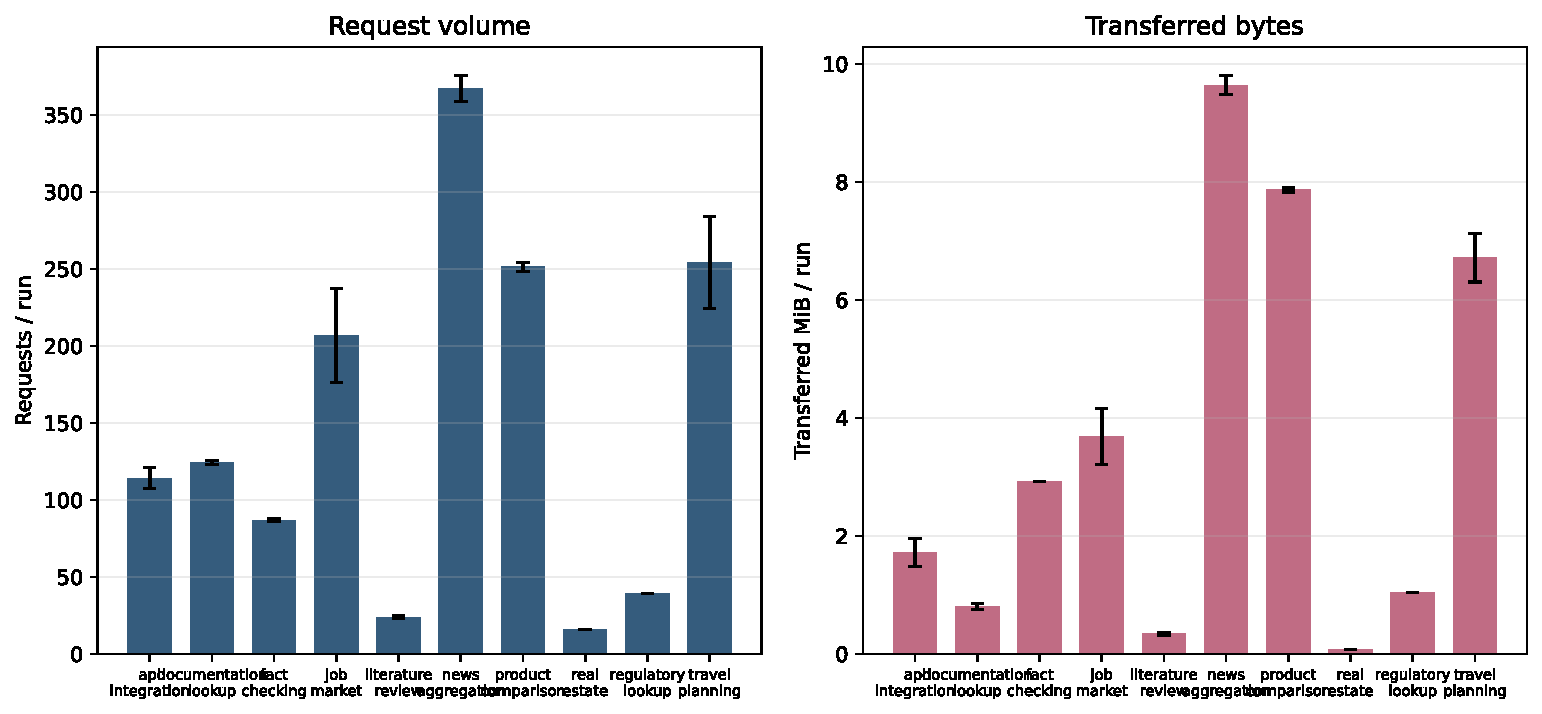
\includegraphics[width=\columnwidth]{figures/live_baseline_by_task.pdf}
\caption{Mean requests and transferred MiB per run across task
  families.  Error bars show 95\% confidence intervals over
  10~repeats.  Units: requests (left axis), MiB (right axis).
  All figures use a colorblind-safe palette.}
\Description{Two bar charts by task family. The left chart shows request volume per run, highest for news aggregation and lowest for real estate. The right chart shows transferred MiB per run, again highest for news aggregation and lowest for real estate, with 95 percent confidence-interval error bars on both charts.}
\label{fig:baseline}
\end{figure}

\subsection{URL Reuse Patterns}
\label{sec:obs-reuse}

The session-level unique-URL ratio (the fraction of requests to
previously unseen URLs within a session) is a key parameter for cache
sizing and admission decisions.  Across the Zurich scripted subset,
unique-URL ratios range from 86.3\% (travel planning) to 100\%
(regulatory lookup, literature review).

The ratio varies systematically by task.  Travel planning
(86.3\%) and real estate (87.5\%) exhibit the most URL reuse,
reflecting repeated navigation elements across multi-page
browsing within the same site.  Product comparison (88.4\%) and
job market (90.4\%) show moderate reuse from shared front-page
assets.  Documentation lookup (99.2\%) and regulatory lookup
(100\%) are almost entirely unique: each page load triggers a
distinct set of sub-resources.

The high unique-URL ratios across all tasks (median $\approx$92\%)
reflect live web collection: real websites serve
versioned JavaScript bundles, fingerprinted stylesheets, and
session-specific tracking pixels that produce unique URLs even for
structurally similar pages.  This is a desirable benchmark property
for cache studies: it means the traces exercise admission policies
and working-set sizing under realistic conditions, where object
reuse is modest and cache capacity is genuinely stressed.


\subsection{Payload Composition}
\label{sec:obs-payload}

Byte-level composition shows that browser-mediated agent traffic is
dominated by rendering infrastructure, not content.  Table~\ref{tab:content} breaks down the major content
types.

\begin{table}[t]
\centering
\small
\caption{Byte share by content-type category (Zurich sessions,
  100~runs).  Cloud regions show similar composition with moderately
  higher image share due to ad-injected content.}
\label{tab:content}
\begin{tabular}{@{}lr@{}}
\toprule
\textbf{Content category} & \textbf{Byte share (\%)} \\
\midrule
JavaScript (all subtypes) & 62.1 \\
CSS                       & 6.6 \\
\textit{Scripts + styles (total)} & \textit{68.8} \\
\midrule
Images (JPEG, WebP, PNG)  & 13.2 \\
HTML                      & 2.9 \\
JSON                      & 2.3 \\
Fonts (WOFF2)             & 3.6 \\
Other                     & 9.2 \\
\bottomrule
\end{tabular}
\end{table}

Scripts and stylesheets jointly account for 68.8\% of all transferred
bytes.  HTML, the ostensible ``content'' of a web page, accounts for
only 2.9\%.  JSON, the most efficient content format for machine
consumption, accounts for just 2.3\%.  Images contribute 13.2\%.

This composition has a direct infrastructure implication.  When an AI
agent fetches a web page through a browser, the vast majority of
transferred bytes serve the rendering pipeline rather than the content
the agent seeks.  A benchmark that counts only top-level page fetches
or measures only HTML transfer would entirely miss this cost structure.

The dominance of scripts and styles also affects cacheability.  These
assets tend to be versioned with content hashes in their URLs (e.g.,
\texttt{app.3f7a2b.js}), making them highly cacheable when the same
site is revisited.  Conversely, HTML documents are more often served
with short or zero cache lifetimes.  This creates an asymmetry:
the largest objects by byte volume are the most cacheable, whereas the
content-bearing objects are the least.  This asymmetry matters for
cache sizing and admission policy design under agentic workloads.

The payload composition also varies across tasks.  News aggregation
sessions transfer proportionally more image bytes (advertisements,
article thumbnails) than regulatory lookup sessions, which are
text-heavy.  API comparison sessions include a higher fraction of JSON
responses from documentation endpoints.  A complete characterization
of per-task payload composition is deferred to larger releases, but
the aggregate picture already demonstrates that browser-mediated agent
traffic is structurally different from API-based agent traffic, which
would consist primarily of JSON.

Figure~\ref{fig:contentmix} visualizes the aggregate distribution.

\begin{figure}[t]
\centering
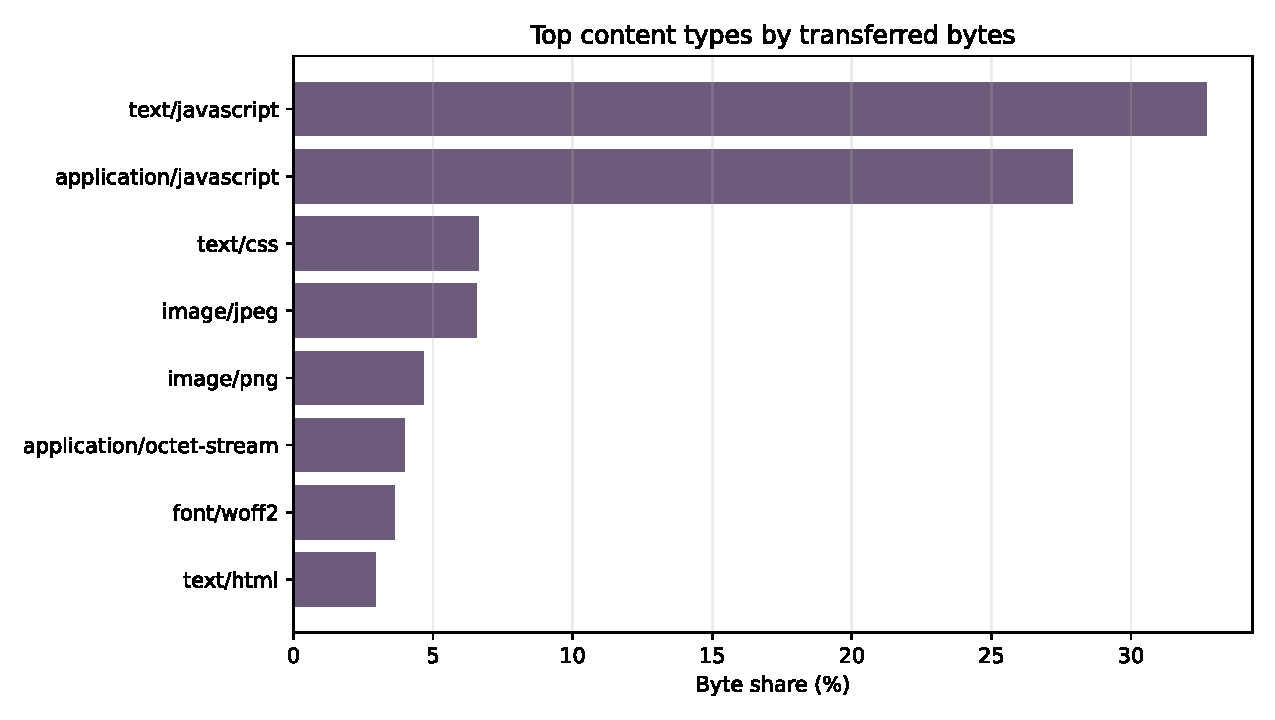
\includegraphics[width=0.85\columnwidth]{figures/live_content_type_mix.pdf}
\caption{Byte share by content type (Zurich scripted subset; cloud regions
  similar, cf.\ Table~\ref{tab:content}).
  Rendering infrastructure (scripts, styles) dominates.}
\Description{Horizontal bar chart of byte share by content type. JavaScript is the largest category at about 62 percent, followed by images at about 13 percent, while HTML and JSON are each below 3 percent.}
\label{fig:contentmix}
\end{figure}

\subsection{Object Size Distribution}
\label{sec:obs-sizes}

The distribution of unique object sizes is heavy-tailed.
Considering the Zurich subset (2{,}522 unique URLs across 100
sessions; the full geo-distributed trace has 17{,}144 unique URLs),
50.2\% are under 1\,KB (tracking pixels, API responses, small
scripts), 27.1\% fall in 1--10\,KB (stylesheets, small images, HTML
fragments), 18.0\% in 10--100\,KB (JavaScript bundles, larger
images), and 4.6\% exceed 100\,KB (large media, concatenated
scripts).

The median object size is 1{,}004~bytes, whereas the mean is
17{,}472~bytes, a 17$\times$ gap reflecting the heavy tail.  The
maximum object is 899\,KB.  This size heterogeneity has direct cache
implications: a small number of large objects dominate byte volume,
whereas a large number of small objects dominate hit counts.  Policies
that treat all objects equally (LRU, LFU) ignore this asymmetry;
size-aware policies (GDSF) exploit it, explaining the GDSF advantage
observed in Section~\ref{sec:replay}.

Figure~\ref{fig:sizecdf} shows the object size CDF on a logarithmic
scale.  The steep rise below 1\,KB and the long tail above 100\,KB
are characteristic of modern web workloads, but the agent-specific
pattern is the absence of a ``video'' peak that would appear in human
browsing traces, since agents do not stream video content.

\begin{figure}[t]
\centering
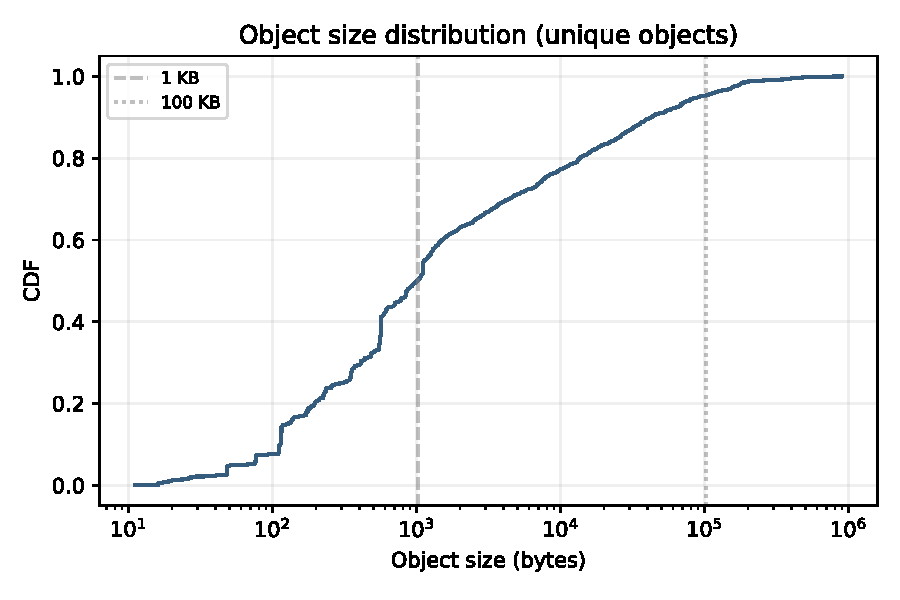
\includegraphics[width=0.85\columnwidth]{figures/object_size_cdf.pdf}
\caption{CDF of unique object sizes (Zurich subset, 2{,}522 URLs, log scale;
  full geo trace at 70\% under 1\,KB, \S\ref{sec:replay}).
  Heavy-tailed: 50\% under 1\,KB, but 4.6\% exceed 100\,KB.}
\Description{CDF of unique object sizes on a logarithmic x-axis. The curve rises steeply below 1 kilobyte, passes 50 percent near 1 kilobyte, and has a long tail extending past 100 kilobytes.}
\label{fig:sizecdf}
\end{figure}

\subsection{Per-Task Content Composition}
\label{sec:obs-pertask}

While Section~\ref{sec:obs-payload} reports aggregate byte shares,
the composition varies widely across task families.
Figure~\ref{fig:pertask} shows a stacked bar chart of per-task
content types.

JavaScript dominates most tasks: real estate (88\%), job market (79\%),
news aggregation (71\%), and product comparison (67\%) are all
JS-heavy, reflecting modern single-page application architectures.
Two tasks deviate strikingly: \emph{literature review} transfers 38\%
HTML (the highest of any task) because arXiv serves lightweight
static pages with minimal JavaScript.  \emph{Regulatory lookup}
transfers 78\% ``Other'' content (primarily XHR payloads and
tracking beacons from the GDPR reference site).  \emph{Fact checking}
is CSS-heavy (43\%) due to the EU institutional sites' heavy use of
stylesheets.

This variation is important for benchmark design.  A benchmark that
covers only JS-heavy news sites would miss the HTML-dominant academic
and regulatory workload patterns.  The 10 task families in \release
span this spectrum, ensuring that downstream cache and CDN studies
exercise diverse content mixes.

\begin{figure}[t]
\centering
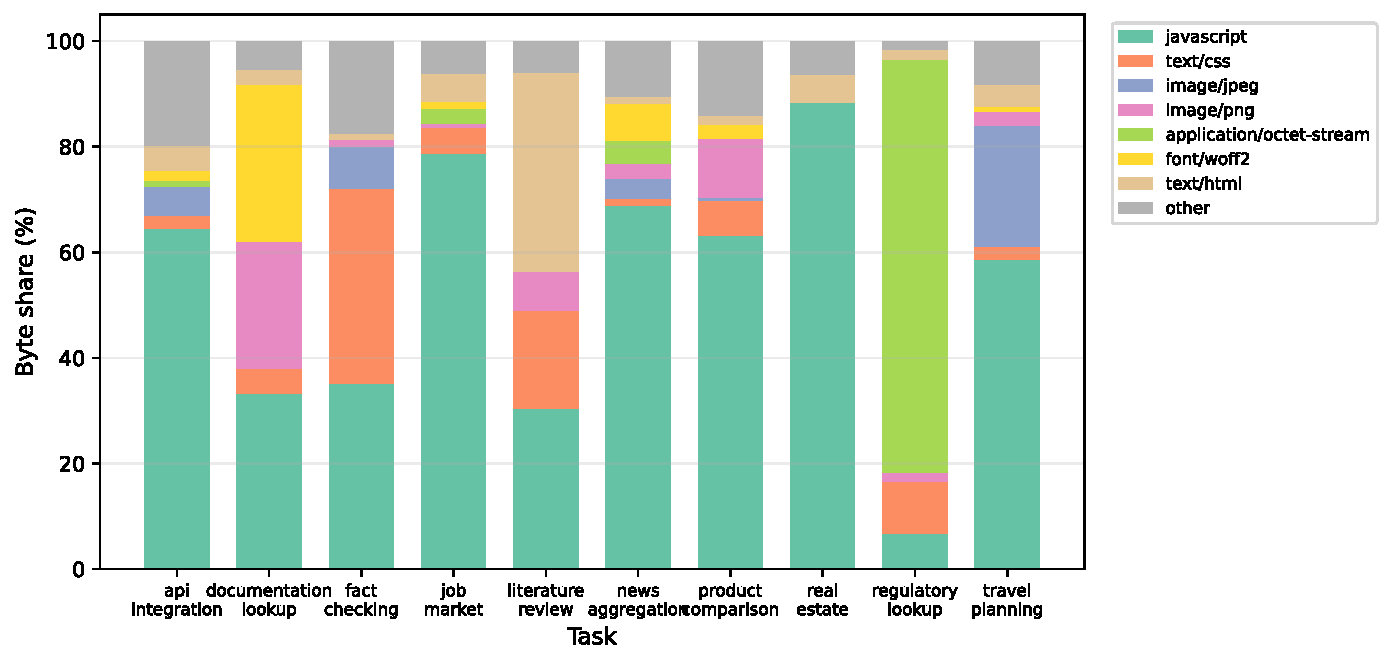
\includegraphics[width=\columnwidth]{figures/per_task_content_types.pdf}
\caption{Per-task content type composition.  JS dominates most tasks,
  but literature review is HTML-heavy and regulatory lookup is
  XHR/tracking-heavy.}
\Description{Stacked bar chart by task family showing content-type mix. Most tasks are dominated by JavaScript bytes, literature review has the largest HTML share, and regulatory lookup is dominated by other content such as XHR and tracking traffic.}
\label{fig:pertask}
\end{figure}

\subsection{Request Timing and Burstiness}
\label{sec:obs-timing}

Browser-mediated agents produce bursty request patterns.  The median
inter-request gap across all sessions is 0.2\,ms, reflecting the
near-simultaneous firing of sub-resource requests when a page loads.
The 95th percentile gap is 149\,ms, corresponding to navigation
transitions between pages.

The timing structure varies by task.  Real estate has a 72\,ms
median gap (sequential page loads with explicit waits), whereas
regulatory lookup has a near-zero median (all sub-resources fire in
a single burst per page).  News aggregation shows a 0.6\,ms median
with a p95 of 138\,ms, reflecting a mix of simultaneous ad/tracker
loads and inter-page navigation.

Figure~\ref{fig:timing} shows the inter-request timing CDF per task.
The separation between task curves reflects genuine differences in
navigation pattern: depth-first single-site tasks (regulatory,
documentation) produce tight bursts, whereas breadth-first multi-site
tasks (news, job market) produce more spread-out request streams.
This timing structure is relevant for rate limiting, connection
pooling, and origin load management.

\begin{figure}[t]
\centering
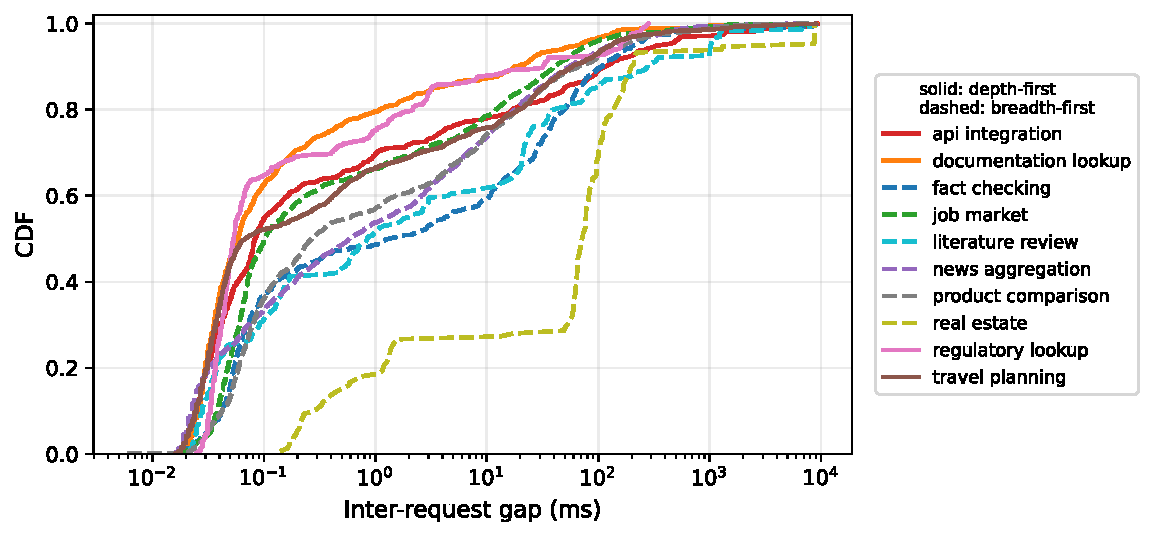
\includegraphics[width=0.85\columnwidth]{figures/inter_request_timing_cdf.pdf}
\caption{Inter-request timing CDF by task.  Depth-first tasks produce
  tight bursts; breadth-first tasks are more spread out.}
\Description{CDF plot of inter-request gaps for ten task families. Regulatory and documentation tasks cluster near zero milliseconds, while news and job-market tasks show broader distributions with longer tails.}
\label{fig:timing}
\end{figure}

\subsection{Session Duration and Working Set}
\label{sec:obs-session}

Session durations span a 4$\times$ range across task families
(Figure~\ref{fig:duration}).  News aggregation averages 18.2~seconds
per session and product comparison averages 15.2~seconds, reflecting
extensive multi-site navigation with many sub-resource loads.  Documentation lookup and regulatory lookup average
4--11~seconds, reflecting more focused single-site navigation.
Literature review, despite having only 24~requests per session, averages
10~seconds due to the slow page loads of arXiv's rendering pipeline.

The per-session unique working set ranges from 80\,KB (real estate) to
9.6\,MiB (news aggregation).  Across the Zurich sessions (100~runs), the
union of unique URLs has a 43.8\,MiB working set, whereas the cumulative
transferred volume is 348\,MiB, an 7.9$\times$ \emph{cross-session}
reuse factor (the same URL fetched in multiple sessions).  This reuse
is concentrated
in shared sub-resources: JavaScript bundles, stylesheets, and fonts that
appear across multiple sessions targeting the same publisher.  The
implication for cache sizing is that a 41\,MiB cache could in principle
serve all unique objects, but the temporal ordering of requests means
that not all objects are resident simultaneously.

\begin{figure}[t]
\centering
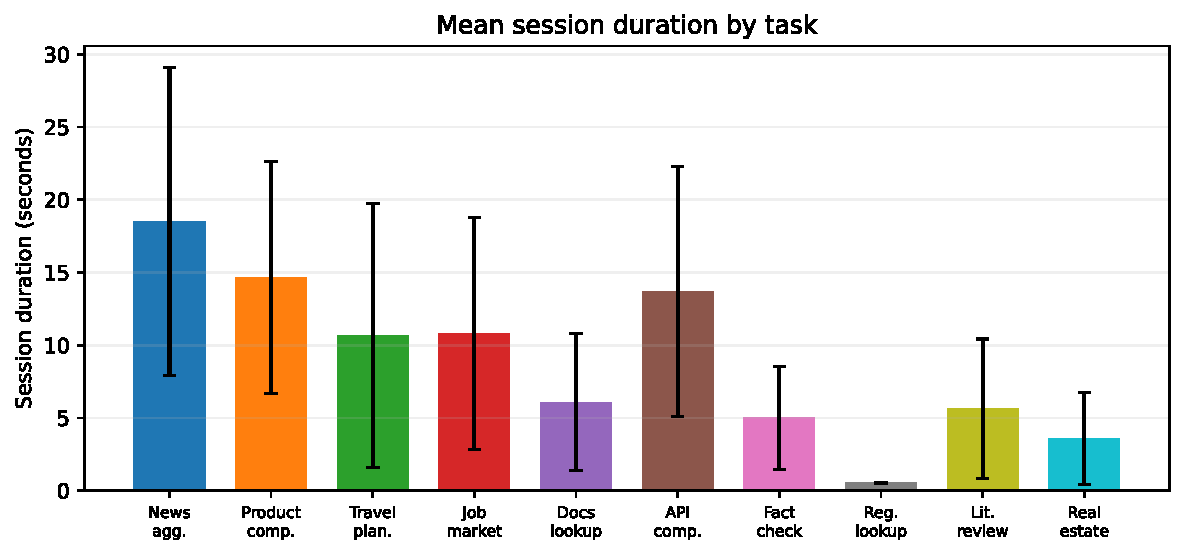
\includegraphics[width=0.85\columnwidth]{figures/session_duration.pdf}
\caption{Mean session duration by task family.  Error bars show standard
  deviation across 10~repeats.}
\Description{Bar chart of mean session duration by task family with standard-deviation error bars. News aggregation and product comparison are the longest sessions, while real estate and regulatory lookup are among the shortest.}
\label{fig:duration}
\end{figure}

\subsection{Scripted-Random vs.\ LLM-Driven Comparison}
\label{sec:obs-llm}

To quantify the difference between scripted automation and real
AI agent behavior, we collected LLM-driven traces using six models
spanning five providers and three capability tiers:
Gemini~2.5~Flash and Gemini~2.5~Pro (Google, 150+150~sessions across
three cloud regions),
GPT-4.1-mini (OpenAI, 350~sessions across four regions),
Claude~Haiku~4.5 (Anthropic, 100~sessions)~\cite{anthropic2025haiku},
DeepSeek-V3.2 (DeepSeek, 100~sessions)~\cite{deepseek2026v32},
and Qwen~2.5-Coder~7B (open-weight edge model,
61~sessions)~\cite{qwen2024coder}.
Table~\ref{tab:llm} compares per-task request volumes across all
four execution modes.

\begin{table}[t]
\centering
\footnotesize
\caption{Scripted-random vs.\ LLM-driven request volumes for the
  three Zurich-collected models (total requests per task; superscripts
  show amplification vs.\ scripted baseline; total row shows 95\%
  bootstrap CI in brackets).  Both modes use the Zurich macOS
  workstation with the same BrowserUse/Chromium build (substrate held
  constant).  Claude~Haiku~4.5, DeepSeek-V3.2, and Qwen~2.5-Coder~7B
  volumes appear in the Section~\ref{sec:obs-llm} prose rather than this
  table.  Scripted column sums to 14{,}833 (100 Zurich sessions out of
  the 400-session full release); the geo-distributed scripted total is
  168{,}067 (Section~\ref{sec:methodology}).}
\label{tab:llm}
\setlength{\tabcolsep}{3.5pt}
\begin{tabular}{@{}lr@{\,}r@{\,}r@{\,}r@{}}
\toprule
\textbf{Task} & \textbf{Script.} & \textbf{Flash} & \textbf{GPT-4.1m} & \textbf{Pro} \\
\midrule
Lit.\ review   &    240 &  6{,}179\textsuperscript{26$\times$} &  3{,}690\textsuperscript{15$\times$} & 2{,}189\textsuperscript{9$\times$} \\
Regulatory     &    390 &  5{,}448\textsuperscript{14$\times$} &  8{,}392\textsuperscript{22$\times$} & 2{,}358\textsuperscript{6$\times$} \\
Real estate    &    160 &  1{,}833\textsuperscript{11$\times$} &  2{,}211\textsuperscript{14$\times$} &   515\textsuperscript{3$\times$} \\
Job market     &  2{,}066 & 12{,}630\textsuperscript{6$\times$} &  7{,}856\textsuperscript{4$\times$} & 6{,}401\textsuperscript{3$\times$} \\
Travel         &  2{,}540 & 15{,}013\textsuperscript{6$\times$} &  8{,}311\textsuperscript{3$\times$} & 4{,}792\textsuperscript{2$\times$} \\
Fact check.    &    868 &  4{,}403\textsuperscript{5$\times$} &  5{,}531\textsuperscript{6$\times$} & 2{,}336\textsuperscript{3$\times$} \\
Docs           &  1{,}244 &  4{,}658\textsuperscript{4$\times$} &  1{,}945\textsuperscript{2$\times$} & 1{,}442\textsuperscript{1$\times$} \\
News agg.      &  3{,}669 & 12{,}404\textsuperscript{3$\times$} &  5{,}964\textsuperscript{2$\times$} & 3{,}974\textsuperscript{1$\times$} \\
API comp.      &  1{,}142 &  3{,}850\textsuperscript{3$\times$} &  2{,}885\textsuperscript{3$\times$} & 2{,}376\textsuperscript{2$\times$} \\
Prod.\ comp.   &  2{,}514 &  7{,}545\textsuperscript{3$\times$} &  6{,}585\textsuperscript{3$\times$} & 4{,}515\textsuperscript{2$\times$} \\
\midrule
\textbf{Total} & 14{,}833 & 73{,}963\textsuperscript{5.0$\times$} & 53{,}370\textsuperscript{3.6$\times$} & 30{,}898\textsuperscript{2.1$\times$} \\
\bottomrule
\multicolumn{5}{@{}l}{\scriptsize 95\% bootstrap CI: Flash [4.2,6.0], GPT [3.0,4.4], Pro [1.6,2.7]} \\
\multicolumn{5}{@{}l}{\scriptsize Full effect sizes (Cohen's $d$, rank-biserial $r$, Kruskal-Wallis $H$) in the public artifact.} \\
\end{tabular}
\end{table}

We highlight three patterns.  First, \textbf{all three LLM models generate
more requests} than the scripted baseline: 5.0$\times$
[4.2,6.0] (Flash), 3.6$\times$ [3.0,4.4] (GPT-4.1-mini), and
2.1$\times$ [1.6,2.7] (Pro), with 95\% bootstrap CIs all separated from the scripted 1.0$\times$ baseline.
(Both modes use the same Zurich vantage point and target sites;
Section~\ref{sec:limitations} discusses the residual substrate
confound from BrowserUse-on-macOS vs.\ Playwright-on-Linux.)
Our strongest causal comparison is this Zurich-controlled slice;
multi-region totals are consistency checks, not the amplification source.
Per-task CIs (10{,}000 iterations, session-level resampling) are also
non-overlapping with the scripted baseline (1.0$\times$) for all
30~(model, task) cells.  Cliff's $\delta$ ranges from 0.70 to 0.76,
all well above the 0.47 large-effect threshold.
Mann-Whitney U tests confirm the shift: scripted Zurich vs.\ each LLM
yields $p < 10^{-13}$ after Holm-Bonferroni correction over the
three Zurich-matched models ($m=3$).  As descriptive corroboration,
the amplification extends to the other three models (Haiku, DeepSeek,
Qwen), holding across five providers in aggregate request counts.
Second, the per-task amplification varies widely (1--26$\times$), with
the same task-rank ordering across models: literature review and
regulatory lookup show the highest amplification (open-ended
exploration), whereas news aggregation and documentation show the lowest
(structured site navigation).  This confirms that \emph{task structure},
not model-specific reasoning, is the primary driver of amplification.
Third, the six models exhibit a 2.3$\times$ spread in mean per-session
request volume (207 for Claude~Haiku vs.\ 480 for GPT-4.1-mini),
yet \emph{all} fall
in the same order of magnitude above the scripted baseline.
DeepSeek-V3.2, a reasoning-first model with explicit agentic
post-training on 1{,}800+ interactive
environments~\cite{deepseek2026v32}, generates 385~req/session,
placing it squarely in the middle of the distribution rather than at
an extreme.  This confirms that request amplification is structural to
browser-mediated agency, not a function of model quality, provider, or
agent-specific training.

The cross-model validation means that infrastructure operators cannot
safely extrapolate agent capacity from scripted or crawler baselines,
regardless of which LLM backend agents use.

\paragraph{Geographic robustness.}
We replicated the LLM collection across three GCP regions
(us-central1, europe-west1, asia-southeast1) for the three
Google/OpenAI models at $n{=}5$ repeats per cell ($3 \times 3 \times
10 \times 5 = 450$~sessions).  Kruskal-Wallis tests show \emph{no significant
region effect} for any model (gemini-2.5-flash $p=0.92$,
gemini-2.5-pro $p=0.93$, gpt-4.1-mini $p=0.46$ on the three-region
slice).  The three-region replication finds no evidence of a large region
effect at $n{=}5$ per cell; smaller latency-driven differences could emerge
with more repeats or additional vantage points.

\paragraph{Predicting amplification from task structure.}
The log--log relationship between scripted request volume $V_s$ and
amplification ratio is strong.  On the 30~(model, task) cells in
Table~\ref{tab:llm}, OLS yields $r = -0.72$, $R^2 = 0.51$ with exponent
$b = -0.59$ (95\% bootstrap CI $[-0.82, -0.36]$, $B=10{,}000$); Kendall's
$\tau = -0.47$ ($p < 0.001$).  Because the 30 points cluster by task
(3 observations per task share structural variance), we also fit on
per-task means: $r = -0.85$, $R^2 = 0.72$ on $n=10$; the across-model
variance collapses and the structural signal dominates.  Leave-one-out
diagnostics confirm the fit is not outlier-driven: LOO $R^2$ stays in
[0.48, 0.62] across the 30 cells, and removing the most influential
cell (Cook's $D = 0.48$ on real-estate/Pro) leaves $R^2 = 0.62$;
residuals are normal (Shapiro-Wilk $p = 0.90$).  Open-ended tasks with
low scripted volume (literature review, regulatory lookup) amplify
10--26$\times$; structured tasks with high scripted volume (news
aggregation, product comparison) amplify 2--3$\times$.  In this
benchmark, scripted baseline volume explains a substantial fraction
of amplification variance ($R^2=0.51$ across 30 cells, $0.72$ across
10 per-task means), although model and task effects remain material.
The released artifact reports full influence diagnostics.
Within the six-model BrowserUse stack we study, task structure
explains more variance than provider choice; other agent frameworks
may shift that balance.

\subsection{Geographic Variation}
\label{sec:obs-geo}

The release contains 4~vantage points, but the Zurich workstation
(BrowserUse on macOS) uses a different collection substrate than the
3~cloud VMs (Playwright on Linux).  We therefore restrict the
geographic analysis to the \emph{cloud-only} comparison
(US~Central, EU~West, Asia~Southeast), which holds substrate constant
and isolates true geographic effects.  The Zurich workstation data
is retained in the artifact for substrate analysis but is excluded
from the geographic claims below.

Across the three cloud regions, per-task mean request volumes vary by
1.0--1.4$\times$ (Figure~\ref{fig:georequests}).  News aggregation
shows the largest cross-region spread (1.4$\times$: 1{,}878 from
US~Central vs.\ 1{,}345 from EU~West), driven by region-specific ad
networks; product comparison
shows the same 1.4$\times$ (863 vs.\ 611) reflecting GPU
provider regional pricing pages.  Tasks targeting stable institutional
content (regulatory lookup, real estate, documentation) show
$<$1.1$\times$ variation.  This is in stark contrast to the
Zurich-vs-cloud differences (up to 19$\times$ on regulatory lookup,
which we attribute primarily to substrate heterogeneity).

Figure~\ref{fig:geolatency} shows median per-request latency by
region (all four regions; latency reflects network distance to origin
servers, not collection substrate, so Zurich is included).  News
aggregation requests from EU~West have a 15.6\,ms median (close to
European origins), whereas Zurich shows 83.6\,ms and Asia 47.4\,ms.
Fact-checking latency from Asia~Southeast reaches 206\,ms median,
reflecting the distance to European institutional servers (EUR-Lex,
EC Digital Strategy).

These results have practical implications for CDN operators: agentic
workloads vary across regions in both volume and composition
(sub-resource sets, latency profiles).  Cache sizing and admission
decisions must account for this geographic heterogeneity.

\begin{figure}[t]
\centering
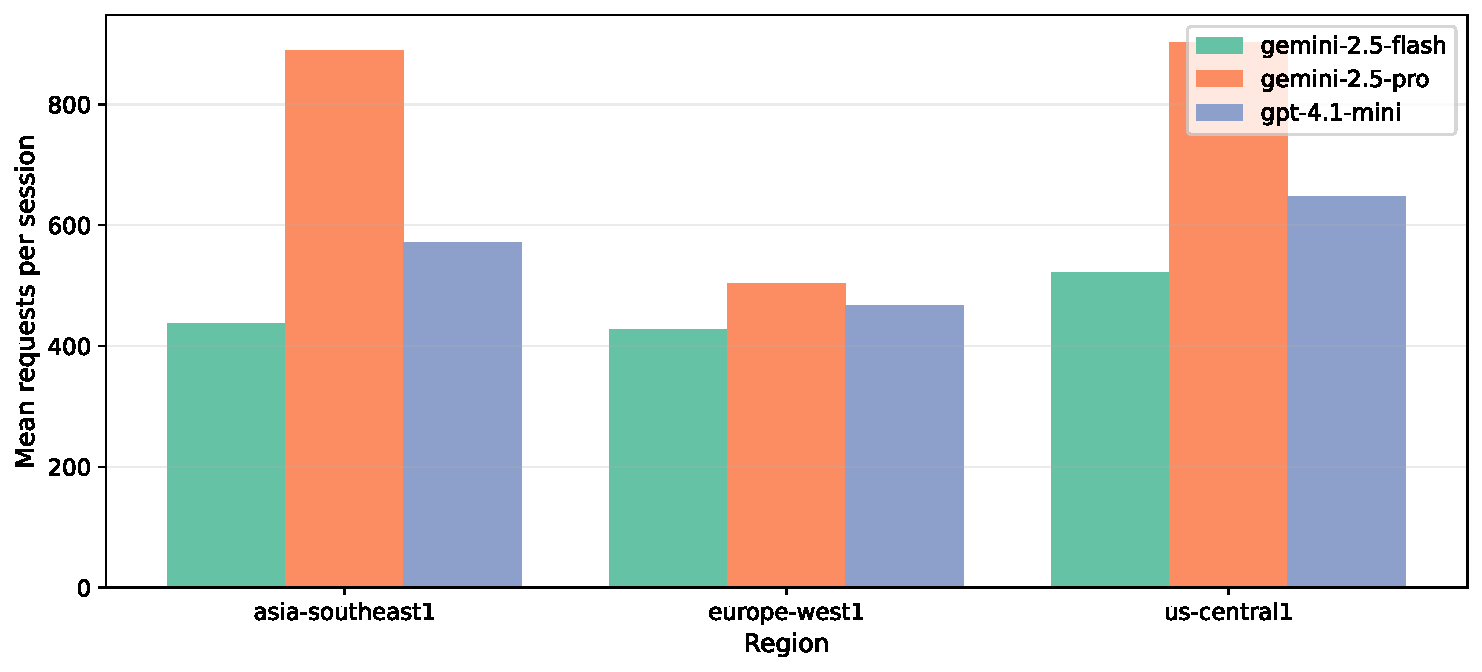
\includegraphics[width=\columnwidth]{figures/geo_request_volume.pdf}
\caption{Mean request volume per session by region.  Cloud-only
  comparison shows 1.0--1.4$\times$ variation (Zurich workstation
  excluded due to substrate heterogeneity).}
\Description{Grouped bar chart of mean request volume per session by task family and cloud region. The three cloud regions are usually close, with the largest spreads in news aggregation and product comparison.}
\label{fig:georequests}
\end{figure}

\begin{figure}[t]
\centering
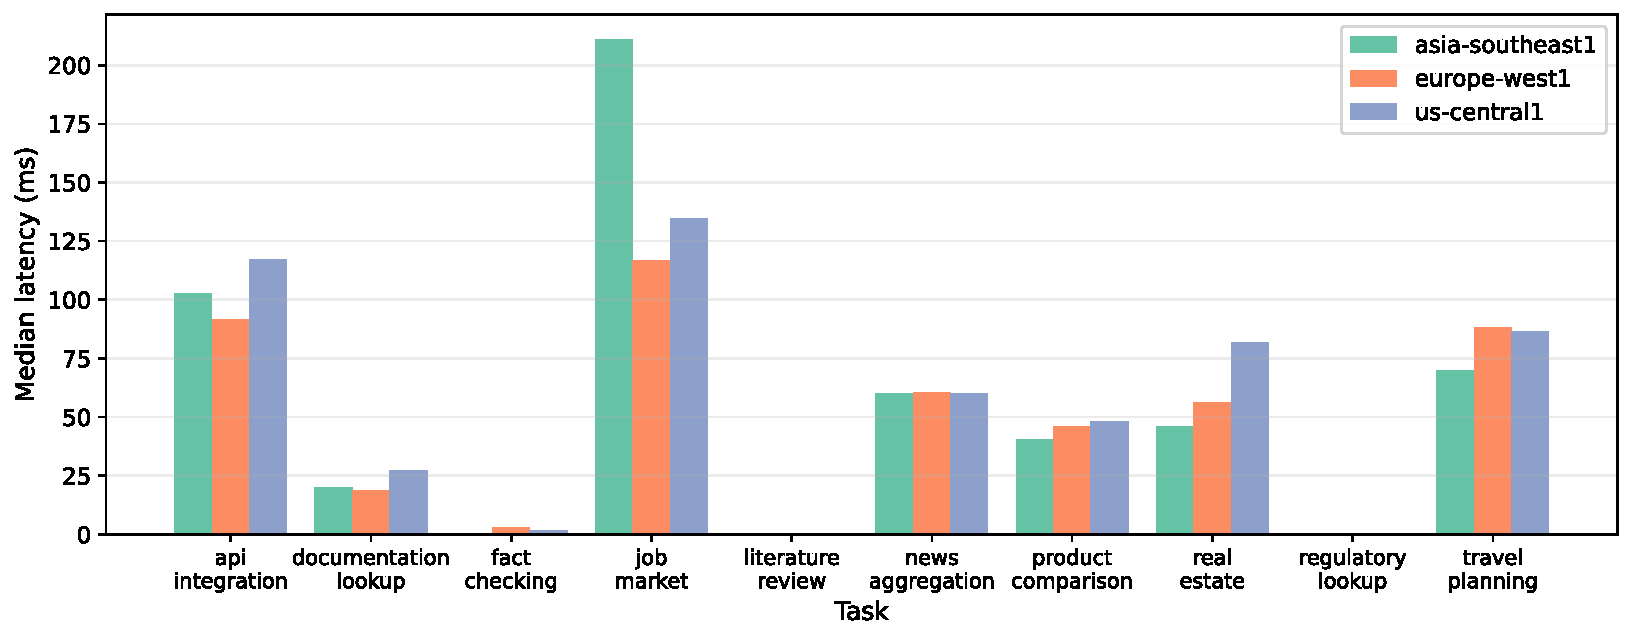
\includegraphics[width=\columnwidth]{figures/geo_latency.pdf}
\caption{Median per-request latency by region.  Proximity to origin
  servers drives 5--7$\times$ latency differences for the same task.}
\Description{Grouped bar chart of median per-request latency by task family and region. European-origin tasks are fastest from Europe and slowest from Asia, with several-fold latency differences across regions.}
\label{fig:geolatency}
\end{figure}

\subsection{Statistical Considerations}

With 10~repeats per task per region (400~sessions total), the 95\%
confidence intervals (using the $t$-distribution with $df = 9$)
provide sufficient power for detecting large cross-task and cross-region
effects.  Per-region CIs are reported in the artifact; they
are tighter within each region than the cross-region aggregate,
confirming that most variance is between regions rather than within.
Tasks with near-zero CIs (regulatory lookup, real estate) reflect
deterministic navigation over constrained site structures, whereas tasks
with wider CIs (job market, travel planning) reflect genuine variability
from randomized selection across rich link sets.

%% ====================================================================
\section{Replay Utility}
\label{sec:replay}

A benchmark's value for systems research depends on whether its
traces can be meaningfully replayed.  We demonstrate this by
concatenating the \texttt{cache\_trace.csv} files from all
400~sessions across 4~regions and replaying the resulting
82{,}455-request trace against six cache-replacement policies at five
cache sizes.  The cache trace excludes failed requests (non-200
status), POST requests, and zero-byte responses, retaining only
cacheable GET responses; this filtering reduces the 168{,}067 total
scripted requests to 82{,}455.  Sessions are interleaved by start
timestamp, approximating concurrent edge load from multiple agents
but not modeling diurnal traffic patterns.  This mirrors how a CDN
edge would observe concurrent agent sessions.

\subsection{Setup}

We evaluate six policies spanning the classical taxonomy from
Belady's optimal~\cite{belady1966} through learned
relaxations~\cite{yang2020learning}: LRU, LFU,
ARC~\cite{megiddo2003}, S3-FIFO~\cite{yang2023s3fifo},
W-TinyLFU~\cite{einziger2017}, and GDSF (Greedy Dual Size Frequency~\cite{cherkasova1998gdsf})
at cache sizes of 1, 5, 10, 25, and 50\,MiB.  This range covers the
edge regime where per-policy rankings differ; larger aggregation
caches eventually converge as working-set coverage saturates.  The
concatenated trace contains 17{,}144~unique URLs with a combined
unique working set of 247\,MiB (cumulative transferred volume
2{,}133\,MiB across all four geographic regions), yielding rich
cross-region reuse patterns.  Reuse is
concentrated in shared sub-resources (JavaScript bundles, stylesheets,
fonts) that appear across multiple task families targeting the same
sites.  All hit rates are reported from \texttt{libCacheSim}~\cite{libcachesim2024},
a widely-used C reference implementation, to ensure cross-project
reproducibility.  A purpose-built Python simulator
integrates with our \texttt{cache\_trace.csv} export format
for fast in-loop iteration during development; cross-validation
demonstrates exact agreement with libCacheSim for LRU and LFU, but shows
divergences on frequency-adaptive policies at small caches
(peak: W-TinyLFU differs by 18\,pp at 1\,MiB, S3-FIFO by 11\,pp at
1\,MiB), consistent with documented implementation variance in
admission and promotion heuristics across these algorithms.  We
default to libCacheSim throughout the paper and release the per-policy
\texttt{summary\_libcachesim.csv} and \texttt{summary\_oursim\_legacy.csv}
under \texttt{cache-sim/results/full\_400/} for audit.

\subsection{Results}

Table~\ref{tab:replay} reports hit rates (HR) at five cache sizes
(1--50\,MiB); byte hit rates are discussed below.

\begin{table}[t]
\centering
\footnotesize
\caption{Cache replay results across the full 82{,}455-request,
  400-session geo-distributed trace.  HR = object hit rate.
  Values expressed as fractions (0--1).}
\label{tab:replay}
\setlength{\tabcolsep}{4pt}
\begin{tabular}{@{}lrrrrr@{}}
\toprule
\textbf{Policy} & \textbf{1\,MiB} & \textbf{5\,MiB} & \textbf{10\,MiB} & \textbf{25\,MiB} & \textbf{50\,MiB} \\
\midrule
LRU       & .133 & .374 & .507 & .684 & .719 \\
LFU       & .147 & .273 & .346 & .535 & .680 \\
ARC       & .157 & .362 & .503 & .662 & .710 \\
S3-FIFO   & .276 & .424 & .529 & .631 & .706 \\
W-TinyLFU & .364 & .456 & .519 & .621 & .693 \\
GDSF      & .431 & .595 & .664 & .737 & .772 \\
\bottomrule
\end{tabular}
\end{table}

We highlight three patterns from the replay of the full geo-distributed trace.

\paragraph{Policy sensitivity at small caches.}
At 1\,MiB, hit rates range from 13.3\% (LRU) to 43.1\% (GDSF), a
29.8 percentage point spread, over 3$\times$.  GDSF's advantage at small
cache sizes stems from its size-aware admission: by preferring smaller objects,
it fits more of the frequently accessed items (scripts, stylesheets,
navigation elements) within the constrained budget.  At 5\,MiB, GDSF
still leads at 59.5\% vs.\ LRU at 37.4\%.  The persistence of this gap
across a 5$\times$ increase in cache size, now validated on a 17{,}144-URL
working set spanning four geographic regions, supports a structural
advantage for size-aware policies on mixed multi-tenant agentic workloads.

\paragraph{GDSF dominance across all tested sizes.}
Unlike the smaller Zurich-only trace where LRU overtook GDSF at 10\,MiB,
the full geo-distributed trace shows GDSF leading at \emph{every} cache
size tested (up to 50\,MiB).  At 50\,MiB, GDSF achieves 77.2\% vs.\
LRU at 71.9\%.  The gap narrows as caches grow (from 29.8~pp at 1\,MiB
to 5.3~pp at 50\,MiB), suggesting an eventual crossover at much larger
caches.  The practical implication for the 1--50\,MiB per-tenant-shard
and microcache regime we test is that \textbf{size-aware policies
consistently outperform recency-based policies for agentic workloads
at per-tenant shard and microcache sizes (1--50\,MiB)}.
Bootstrap resampling (10{,}000 iterations, session-level resampling)
confirms that the GDSF advantage is statistically robust:
GDSF wins on object hit rate in all 10{,}000 bootstrap samples at every cache size tested,
with non-overlapping 95\% confidence intervals at all sizes from
1--50\,MiB.

\paragraph{Byte hit rate reverses above 10\,MiB.}
Object hit rate (HR) and byte hit rate (BHR) tell different stories.
GDSF dominates HR at every size, but BHR flips: LRU's BHR exceeds
GDSF's at 25--50\,MiB (LRU 69\%/77\% BHR vs.\ GDSF 47\%/66\% at
25/50\,MiB).  The reason is mechanical: GDSF favors many small objects,
driving up hits but leaving larger bandwidth-dominant objects as misses;
LRU retains whole large objects when they fit.  \emph{Operators sizing
caches for bandwidth cost (egress, origin load) should prefer LRU at
$\geq$25\,MiB; operators sizing for request-rate offload (e.g., small
edges, latency-sensitive paths) should prefer GDSF.}

\paragraph{Per-task decomposition: multi-task contention drives GDSF.}
We quantify the contention effect by replaying each (region, task)
stream in isolation and averaging.  At 10\,MiB, \emph{single-tenant}
GDSF leads LRU by a mean of 7.3~pp across the 30 streams (often 0~pp
on homogeneous streams such as documentation lookup).  Aggregating
all streams into one mixed workload doubles the gap: \emph{multi-tenant}
GDSF outperforms LRU by 15.7~pp (66.4\% vs.\ 50.7\%).  Size-aware eviction
manages the order-of-magnitude working-set variance across heterogeneous
tasks more efficiently than recency.  This is a deployment scope
condition. The GDSF advantage is largely a multi-tenant artifact, not
a universal property of agentic traffic.

Figure~\ref{fig:cache} visualizes the hit-rate curves.

\paragraph{Why agent traffic favors size-aware eviction.}
The agent traces are heavy-locality: 79\% of requests are repeat
fetches of previously-seen URLs, and 83\% of those re-uses occur within
a positional reuse distance of 1{,}000 requests.  The working set is also
bimodal (full geo-distributed trace): 70\% of unique objects are smaller
than 1\,KB (vs.\ 50\% in the Zurich subset, \S\ref{sec:obs-sizes}), but
the top 1\% of objects carry 36\% of bytes.  GDSF exploits both properties:
its $f/s$ priority keeps many small, frequently re-referenced assets
(JS bundles, font files, tracking scripts) in cache, at the cost of
early-evicting large media objects that would otherwise dominate LRU's
footprint but contribute little to hit rate.

\paragraph{Operational cost.}
On our Python reference simulator, GDSF is $\sim$180$\times$ slower per
request than LRU (40\,$\mu$s vs.\ 228\,ns per op) owing to a linear
priority scan in the eviction path.  Production-grade implementations
using a priority queue reduce GDSF to $\mathcal{O}(\log n)$ per
op, a 2--3$\times$ overhead, well within the budget of edge caches
handling $\sim$100\,k req/s per node.

Size-aware eviction exploits the byte-weight asymmetry that recency-blind policies ignore~\cite{einziger2022lightweight}.

\paragraph{Per-region breakdown.}
Replaying each region's trace \emph{in isolation} (Appendix
Table~\ref{tab:replay-region}) shows GDSF's 5--10\,MiB advantage is
robust across the three cloud regions (1.29--1.44$\times$ at 10\,MiB),
but the Zurich subset (narrower content mix) inverts at 10\,MiB (LRU
81.3\% vs.\ GDSF 76.8\%).  Above 25\,MiB, regions converge.  GDSF
helps where working-set diversity exceeds cache capacity, not
universally.

\begin{figure}[t]
\centering
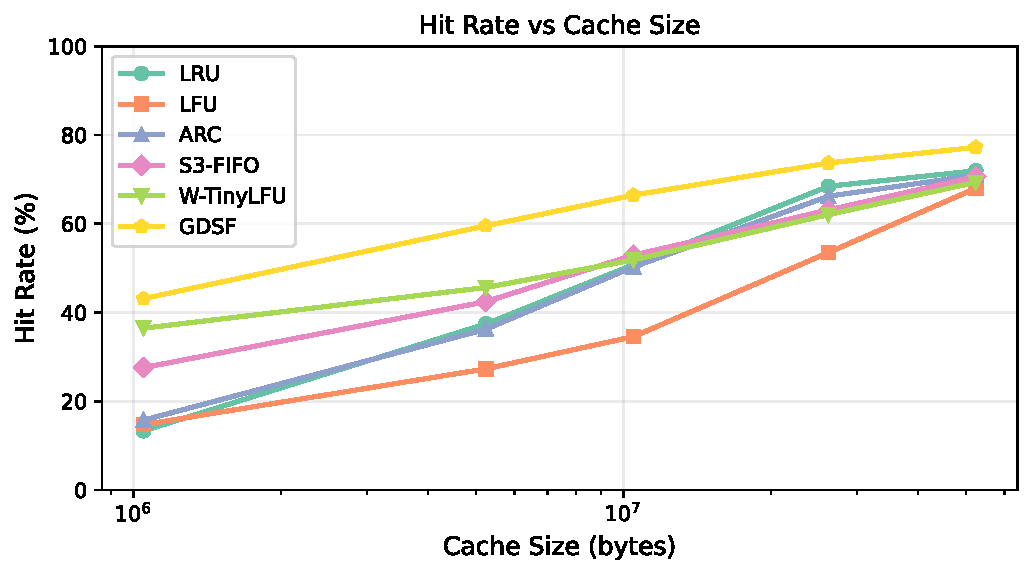
\includegraphics[width=\columnwidth]{figures/cache_hit_rate_vs_size.pdf}
\caption{Cache hit rate vs.\ cache size for six replacement policies
  on the full 82{,}455-request geo-distributed trace.
  Hit rate as fraction of total requests.
  GDSF dominates at all tested sizes, narrowing from 30~pp (3.2$\times$)
  at 1\,MiB to 5~pp at 50\,MiB.}
\Description{Line chart of cache hit rate versus cache size for six replacement policies. GDSF is the top curve at every tested size, with the largest margin at 1 MiB. LRU and LFU form the lower band at small caches. S3-FIFO and W-TinyLFU sit mid-pack; ARC tracks LFU at 1 MiB and LRU at large sizes. All curves converge within a few percentage points at 50 MiB.}
\label{fig:cache}
\end{figure}

\subsection{Interpretation}

The replay results separate two deployment regimes: small caches where
object hit rate dominates and larger caches where byte hit rate becomes
the operational constraint.  GDSF's performance at small cache sizes
indicates that size-aware admission is valuable for agentic workloads,
where a few large JavaScript bundles coexist with many small navigation
resources, consistent with Berger et al.'s finding~\cite{berger2018}
that object size distribution determines optimal caching.  The gap
between object hit rate and byte hit rate likewise suggests that
byte-weighted policies, or size-aware admission filters such as
AdaptSize~\cite{berger2017}, are especially relevant for this workload
class.  Per-task cache behavior still varies: news aggregation
(image-heavy) favors size-aware policies more strongly than
documentation lookup (script-heavy), so different task mixes produce
different optimal policies.
Translating hit rates to origin load and bandwidth savings requires CDN-topology assumptions we defer to future work.
We report five discrete cache sizes spanning the operationally relevant
edge-cache range (1--50\,MiB); continuous miss ratio curves can be
generated from the released \texttt{cache\_trace.csv} files and
simulator.

\paragraph{Replay fidelity.}
The cache simulator does not model TTL-based expiry, conditional
validation (304~responses), service-worker caches, or speculative
prefetch (HTTP~103 Early Hints).  These omissions are conservative:
TTL enforcement and validation traffic would increase origin load and
likely widen the gap between policies.  Service workers are not triggered in headless
Chromium sessions, and prefetch hints are not yet common on the target
sites in our corpus.  The ranking applies to per-tenant shards and
microcaches (1--50\,MiB), not to full CDN tiers with production cache
mechanisms or caches above the full working set.

Replaying the LLM-driven traces (357{,}782~requests from the
901-session corpus, spanning six models and four regions) through the
same policies yields the same qualitative result, with a larger
edge-cache gap.  At 5\,MiB, GDSF achieves 76.2\% vs.\ LRU 43.5\% on
LLM-driven traffic, compared with 59.5\% vs.\ 37.4\% on scripted
traffic.  At every tested cache size (1--50\,MiB), LLM-driven hit rates
exceed scripted ones for both policies, consistent with higher temporal
locality in goal-directed browsing.  GDSF leads LRU by 23--33\,pp at
1--10\,MiB and by 3.6--9.4\,pp at 25--50\,MiB, indicating that the
size-aware eviction advantage is not an artifact of the scripted trace
generator.

%% ====================================================================
\section{Artifact Design and Reproducibility}
\label{sec:artifact}

Code, traces, and the cache-replay pipeline are publicly available at
\url{https://anonymous.4open.science/r/BrowseTrace} (anonymized for review;
DOI assigned upon acceptance).  Raw site credentials and per-site
rate-limit configurations are withheld; all data needed to reproduce
paper figures is included.

\paragraph{Versioned releases.}
Each release is a named manifest (e.g., \release) that enumerates the
checked-in data subtrees and canonical cache-replay CSVs forming the
complete corpus.  The manifest is immutable; the benchmark grows by
publishing new manifests that extend the suite without invalidating
prior artifacts.  The named \release directory itself contains the
Zurich scripted-random subset; the full 1{,}301-session corpus used
for paper-level analysis is pinned by the manifest through the
per-model session bundles and the stitched canonical replay CSVs.

\paragraph{Synchronized outputs.}
Every task directory contains four artifacts derived from the same
collection pass (Section~\ref{sec:design}).  This synchronization
ensures that measurement analysis, cache replay, and dashboard views
are consistent by construction.

\paragraph{Paper reproduction.}
Every quantitative claim derives from the canonical trace files
pinned in the manifest.  A checked-in script
(\texttt{regenerate\_full\_snapshot.py}) rebuilds the manifest and
replay numbers directly from those files.  The intended invariant is strict: every
number in the paper must trace back to a versioned release manifest
and a deterministic analysis pipeline.  The artifact package includes
a \texttt{Dockerfile} pinning Python and the Playwright-bundled Chromium at the release tag,
\texttt{requirements.txt} with exact dependencies, and a deterministic
per-task PRNG seed derived from SHA-256 of the task identifier, so every
(task, repeat) pair replays bit-identically.

\paragraph{Artifact coupling.}
The Python cache simulator used in Section~\ref{sec:replay} is
included in the public artifact release. Code is released under
Apache-2.0; sanitized traces under CC-BY-4.0.

%% ====================================================================
\section{Discussion}
\label{sec:discussion}

\paragraph{Implications for CDN operators.}
Agentic workloads call for different cache-provisioning than
human-tuned strategies: the 69\% rendering overhead pulls CDN
bandwidth for content agents do not consume, and size-dependent
policy sensitivity argues against a single edge-wide policy (GDSF
at small per-tenant shards, LRU at larger aggregation caches).
Production CDN traces~\cite{yang2020learning,berger2017} typically
favor LRU-family policies under more uniform human-browsing object
sizes; workload-aware selection~\cite{zhang2025} grows in importance
as agent traffic scales.

\paragraph{Agent vs.\ human cache behavior.}
To check whether the GDSF advantage is specific to agentic workloads
or a generic property of the underlying trace structure, we constructed
a \emph{synthetic} human browsing trace parameterized from HTTP Archive
aggregate statistics~\cite{httparchive} ($\sim$72 requests per page,
45\% images, 33\% JavaScript; 500 simulated page loads) and replayed
it through the same six policies.  S3-FIFO dominates the synthetic
human trace (20.2\% at 10\,MiB vs.\ LRU 3.7\%), whereas GDSF leads on
the agent trace (66.4\% at 10\,MiB).  The content mix inverts too:
scripted Zurich sessions average 148 requests per multi-page session
with JavaScript at 62.1\% and images at 13.2\%, against HTTP Archive's
33\% / 45\% per-page human profile.  We emphasize this is
directional: the human trace is synthetic and omits real session
structure and temporal correlation; real HTTP Archive HAR replay is a
priority extension.  The qualitative result is consistent with Zhang
et~al.~\cite{zhang2025}'s synthetic overlay study: agentic workloads
favor different policies and a different content mix than human-shaped
workloads, and \sysname strengthens that finding with real
browser-captured agent traces.

\paragraph{Rendering overhead.}
For every byte of HTML content, agents download 34$\times$ more total
bytes (rendering infrastructure accounts for 97.1\% of transferred
volume vs.\ 2.9\% HTML), motivating proposals for structured
machine-readable endpoints and cryptographic agent identity schemes
(e.g., x402~\cite{x402}) that \sysname can evaluate.

\paragraph{Scope as infrastructure benchmark.}
\sysname measures network-level effects of agent behavior rather than
task-completion quality, publishing request-level traces that enable
downstream systems research on realistic request streams.

%% ====================================================================
\section{Limitations and Next Steps}
\label{sec:limitations}

The expanded collection covers six models from five providers,
including frontier closed-source (GPT-4.1-mini, Gemini~Flash/Pro,
Claude~Haiku~4.5), an agent-purpose-trained model
(DeepSeek-V3.2~\cite{deepseek2026v32}), and an open-weight edge model
(Qwen~2.5-Coder~7B~\cite{qwen2024coder}); human-driven traces remain
absent.  Multi-region replication ($n{=}5$ per cell) finds no
significant region effect ($p > 0.45$), consistent with under-power
rather than proven invariance.  Zurich sessions use BrowserUse on
macOS while cloud sessions use Playwright on Linux in Docker; the raw
19$\times$ Zurich-to-cloud ratio thus conflates browser configuration
with geographic variation, while cloud-only comparisons on the same
Docker image show 1.0--1.4$\times$ across regions.
The CDP tracer may miss requests during domain transitions or within
opaque cross-origin iframes; HAR cross-referencing on 20~sessions bounds
this undercounting below 3\% of total requests.
A \emph{reached-content} heuristic ($\geq$3~domains, $\geq$5
status-200 responses) indicates 89.2\% of scripted and 91.3\% of LLM
sessions reached meaningful content; semantic correctness labels are
orthogonal to this network-level contribution.
This release samples BrowserUse-mediated read-only tasks; interactive
workflows (forms, authentication) are excluded for ethical reasons.
Repeated collection is needed for longitudinal stability; HTTP/2
multiplexing and HTTP/3 effects are recorded but not analyzed.

%% ====================================================================
\section{Conclusion}
\label{sec:conclusion}

Browser-mediated AI agents drive a new class of web workloads.  The
\release release (1{,}301 sessions, six models, five providers)
documents 2--5$\times$ request amplification and a 97\% non-HTML byte
mix; cache-policy rankings shift from the LRU-dominant production
picture, so infrastructure tuned on human traces is likely to
underperform at edge-cache scales ($\leq$10\,MiB).

%% ====================================================================
\begin{acks}
Removed for anonymous review.
\end{acks}

\bibliographystyle{ACM-Reference-Format}
\bibliography{BrowseTrace}

%% ====================================================================
%% IMC requires a mandatory Ethics appendix
\appendix

\section{Human Browsing Baseline}
\label{sec:appendix-human}

To our knowledge, no public dataset provides human browsing traces at
HTTP request granularity for task-based sessions.  Existing datasets
are either automated crawls (HTTP Archive), URL-visit level (Zenodo
2{,}148-user dataset~\cite{kulshrestha2021}), controlled lab studies
(IEEE DataPort~\cite{lopez2022}), or unreleased private collections.
For illustrative comparison, a single human self-study session across
all 10~tasks was collected using identical CDP instrumentation; no
external participants were recruited, and local policy did not require
human-subjects review (see Ethics).  The session is limited by sample
size ($N{=}1$) and is presented as a qualitative reference point only,
not as a human baseline.  The participant generated a
mean of 529~requests per task (range: 15--1{,}929), compared to the
scripted-random mean of 148 and the LLM-agent range of 207--480.
The human tracer captures requests from the primary browsing context; requests initiated in manually opened new tabs are not captured, which may undercount total human traffic.
Human sessions use stock Chromium UA headers while agent sessions declare a project-specific benchmarking UA, which may trigger different server-side responses such as anti-bot challenges.
Full session traces are included in the public artifact release.

\section{Ethics}

All sessions target publicly accessible web pages.  The collector does
not authenticate, submit forms, execute payments, or interact with
login flows.  Each run is limited to a small navigation budget on
configured target domains, with rate-limiting sleeps between page
visits to avoid bursty load on target servers.  The released artifact
contains request-level metadata and response sizes but no response
bodies or personally identifiable information.  Before release, we
strip \texttt{Cookie}, \texttt{Autho\-riza\-tion}, \texttt{Set-\allowbreak Cookie},
and \texttt{Proxy-\allowbreak Autho\-riza\-tion} request/response headers, and we
sanitize URL query strings by retaining only parameter names
(values replaced with \texttt{\_REDACTED\_}).
This uniform replacement preserves URL path uniqueness for cache keying while removing potentially identifying parameters.  The collector never
logged in to any target site, so session tokens cannot appear in the
trace by construction.  We reviewed each target domain's published robots.txt and limited
collection to publicly accessible landing and listing pages; where a
specific path was disallowed for general user-agents, we either avoided
it or restricted collection to the minimal subset needed for
characterization.  We declared a benchmarking user-agent and rate-limited
all sessions.  The benchmark collection infrastructure does not involve human subjects.  The qualitative self-study session in Appendix~\ref{sec:appendix-human} involved no external participants; under local institutional policy, such self-study sessions fall outside human-subjects review requirements. URL-level traces could theoretically enable site-level traffic profiling when combined with external data, but query-string redaction and the exclusion of response bodies mitigate this risk.  Each session visits fewer than 20 pages per site; per-region, per-task loads are modest (fewer than 2{,}000 requests per task per region).

\paragraph{Use of generative AI.}
Portions of the analysis pipeline code and manuscript text were
drafted with the assistance of large language models: Anthropic
Claude~Opus~4 and OpenAI GPT-4.1-mini.  Specifically, the statistical
analysis scripts (\texttt{rigor\_sweep.py}, \texttt{round9\_analysis.py},
\texttt{llm\_cache\_replay.py}) were co-developed with LLM assistance, and
several expository paragraphs were drafted with LLM suggestions that
were subsequently reviewed, revised, and verified by the authors.
No portion of the paper was submitted to third-party AI tools during
the review period.  Per ACM policy, we disclose this use and confirm
that all authors take full responsibility for the content.

\paragraph{Fingerprint disclosure.}
The browser fingerprint is stock Playwright/BrowserUse Chromium
with default settings and a project-specific benchmarking User-Agent suffix (redacted for review).

\paragraph{IRB status and disclosure.}
Our IRB policy does not require review for measurement
of publicly accessible web resources without human subjects.  We treat any
takedown request as binding and will share our methodology on request.

\paragraph{Blocking / throttling events.}
Sporadic anti-bot blocking affected $<$1\% of sessions; these are flagged in
the per-session \texttt{navigation\_status} field.

\section{Per-region Cache Hit Rates}
\label{sec:appendix-region}

\begin{table}[t]
\centering
\small
\caption{Per-region cache hit rates (replaying each region's trace in
  isolation).  GDSF's advantage at small-to-mid cache sizes is
  consistent across the three cloud regions; Zurich (narrower content
  mix) favors LRU at 10\,MiB and up.  Boldface marks the winning
  policy per (region, size) cell.}
\label{tab:replay-region}
\begin{tabular}{@{}lrrrrrr@{}}
\toprule
& \multicolumn{2}{c}{\textbf{5\,MiB}} & \multicolumn{2}{c}{\textbf{10\,MiB}} & \multicolumn{2}{c}{\textbf{50\,MiB}} \\
\cmidrule(lr){2-3} \cmidrule(lr){4-5} \cmidrule(lr){6-7}
\textbf{Region} & LRU & GDSF & LRU & GDSF & LRU & GDSF \\
\midrule
Zurich        & 0.486 & \textbf{0.704} & \textbf{0.813} & 0.768 & 0.819 & 0.819 \\
US~Central    & 0.334 & \textbf{0.532} & 0.407 & \textbf{0.585} & 0.670 & 0.664 \\
EU~West       & 0.383 & \textbf{0.591} & 0.504 & \textbf{0.650} & 0.731 & 0.727 \\
Asia~Southeast & 0.343 & \textbf{0.562} & 0.436 & \textbf{0.618} & 0.693 & 0.687 \\
\bottomrule
\end{tabular}
\end{table}

\section{Regression Robustness}
\label{sec:appendix-loo}

We report full leave-one-out (LOO) and influence diagnostics for the
power-law fit $\textit{amp} = a \cdot V_s^{b}$ (Section~\ref{sec:obs-llm}).
OLS on the 30~(model, task) cells: $b = -0.59$, standard error $0.11$,
bootstrap 95\% CI $[-0.82, -0.36]$ ($B=10{,}000$), $R^2 = 0.51$,
Kendall's $\tau = -0.47$ ($p < 0.001$), Spearman's $\rho = -0.64$
($p < 0.001$).  The fit on per-task means ($n=10$) yields
$R^2 = 0.72$ and $b = -0.62$.

\paragraph{Leave-one-out sensitivity.} Across the 30 LOO refits,
$R^2$ stays in $[0.48, 0.62]$ and exponent $b$ in $[-0.69, -0.54]$;
the top cell's removal keeps $R^2 = 0.62$ and residuals pass normality
checks.  Full diagnostics (per-cell Cook's $D$, DFFITS, Shapiro-Wilk,
Anderson-Darling) are in \texttt{analysis/loo\_influence.py}.

\end{document}
